\chapter{Classer les êtres vivants}\label{ch:g3:sorting-living-things}

Renverse une boîte de boutons mélangés sur la table, et tes mains se
mettent à \omterm{def:g3:sorting-living-things:criterion}{trier} toutes seules~: les gros avec les gros, les rouges
avec les rouges, ceux à quatre trous avec ceux à quatre trous. Les
naturalistes ont ressenti la même envie devant le fouillis de
scarabées, d'\omterm{prop:g3:sorting-living-things:groups}{oiseaux}, de fougères et de \omterm{prop:g3:sorting-living-things:groups}{poissons} du monde vivant ---
et classer soigneusement les \omterm{def:g1:living-or-not:living}{êtres vivants} s'est révélé l'une des
idées les plus puissantes de la \omterm{def:g1:living-or-not:living}{biologie}.

\section{Classer demande une règle}

\begin{definition}[Trier et critères]\label{def:g3:sorting-living-things:criterion}
\emph{Trier}\index{trier} une collection, c'est mettre ensemble ce
qui va ensemble. Un \emph{critère}\index{critère} est la règle qui
sert au tri --- «~a six pattes~», «~a des \omterm{def:g1:animals-around-us:covering}{plumes}~». Un bon critère
pour les \omterm{def:g1:living-or-not:living}{êtres vivants} est un caractère du corps que l'on peut
\emph{observer}~: quelque chose que l'\omterm{def:g1:animals-around-us:animal}{animal} ou la \omterm{def:g1:plants-around-us:plant}{plante}
\emph{possède}, et non le lieu où il vit ni ce qu'il est en train de
faire.
\end{definition}

\begin{example}[Deux tris des mêmes animaux]\label{ex:g3:sorting-living-things:two}
Prends le chat, le canard, la truite et la coccinelle. Triés selon
«~vit près de l'eau~»~: le canard et la truite ensemble. Triés selon
«~a des \omterm{def:g1:animals-around-us:covering}{plumes}~»~: le canard reste seul. Les deux sont des tris ---
mais seul le second utilise le corps de l'\omterm{def:g1:animals-around-us:animal}{animal}, et c'est le genre
auquel les biologistes se fient~: un \omterm{def:g1:animals-around-us:animal}{animal} peut déménager, il ne
peut pas échanger ses \omterm{def:g1:animals-around-us:covering}{plumes} contre des \omterm{def:g1:animals-around-us:covering}{écailles}.
\end{example}

\begin{remark}[Pourquoi ne pas trier par la maison ou le menu~?]\label{rem:g3:sorting-living-things:why}
Le \omterm{def:g2:where-animals-live:habitat}{milieu de vie} et le menu changent avec les saisons et selon la
chance --- le merle de \cref{ch:g2:what-animals-eat} passe des vers
aux baies sans devenir un autre \omterm{def:g1:animals-around-us:animal}{animal}. Les caractères du corps,
eux, restent. Voilà pourquoi «~ce qu'il possède~» l'emporte sur
«~ce qu'il fait~» comme règle de tri.
\end{remark}

\section{Les grands groupes d'animaux}

\begin{proposition}[Quelques grands groupes]\label{prop:g3:sorting-living-things:groups}
Le tri par caractères du corps rassemble les \omterm{def:g1:animals-around-us:animal}{animaux} en grands
groupes, dont~:
\begin{itemize}
  \item les \emph{insectes}\index{insecte}~: six pattes, un corps
        en trois parties --- la fourmi, la coccinelle, l'abeille, le
        papillon~;
  \item les \emph{poissons}\index{poisson}~: des nageoires et des
        \omterm{def:g1:animals-around-us:covering}{écailles}, une vie passée dans l'eau --- la truite, le
        poisson rouge~;
  \item les \emph{oiseaux}\index{oiseau}~: des \omterm{def:g1:animals-around-us:covering}{plumes}, des ailes et
        un bec --- le canard, le merle, l'autruche~;
  \item les \emph{mammifères}\index{mammifère}~: des poils, et des
        mères qui nourrissent leurs petits de \omterm{def:g2:animals-grow-up:born}{lait} --- le chat, la
        vache, la chauve-souris, la baleine --- et les humains~;
  \item les \emph{amphibiens}\index{amphibien}~: une \omterm{def:g1:the-five-senses:sense}{peau} humide,
        des \omterm{def:g2:animals-grow-up:born}{œufs} pondus dans l'eau, une enfance de têtard --- la
        grenouille, le triton.
\end{itemize}
\end{proposition}
\admitted

\begin{omfigure}
\begin{tikzpicture}
  \foreach \x/\name/\feat in {
      0/insectes/{6 pattes},
      2.95/poissons/{nageoires, écailles},
      5.9/oiseaux/{plumes, bec},
      8.85/mammifères/{poils, lait},
      11.8/amphibiens/{peau humide}} {
    \draw[thick, omDef, fill=omDef!6, rounded corners=5pt]
      (\x,0) rectangle ({\x+2.8},1.7);
    \node[font=\small\bfseries, text height=1.6ex, text depth=0.4ex]
      at ({\x+1.4},1.3) {\name};
    \node[font=\small, text height=1.6ex, text depth=0.4ex]
      at ({\x+1.4},0.6) {\feat};
  }
\end{tikzpicture}

{\small Cinq grands groupes, chacun nommé d'après ce que ses \omterm{def:g1:my-body:parts}{membres}
\emph{possèdent}.}
\end{omfigure}

\begin{example}[Des surprises bien traitées]\label{ex:g3:sorting-living-things:surprises}
Les \omterm{def:g3:sorting-living-things:criterion}{critères} nous épargnent les devinettes paresseuses. La
chauve-souris vole comme un oiseau --- mais elle a des poils, pas de
\omterm{def:g1:animals-around-us:covering}{plumes}, et nourrit ses petits de \omterm{def:g2:animals-grow-up:born}{lait}~: un mammifère. La baleine
nage comme un poisson --- ses poils sont presque réduits à rien,
mais elle a du \omterm{def:g2:animals-grow-up:born}{lait} pour son baleineau et pas d'\omterm{def:g1:animals-around-us:covering}{écailles}~: un
mammifère aussi. L'autruche ne vole pas du tout, et pourtant ses
\omterm{def:g1:animals-around-us:covering}{plumes} et son bec disent~: oiseau. C'est le \omterm{def:g3:sorting-living-things:criterion}{critère} qui décide, pas
l'impression.
\end{example}

\begin{omfigure}
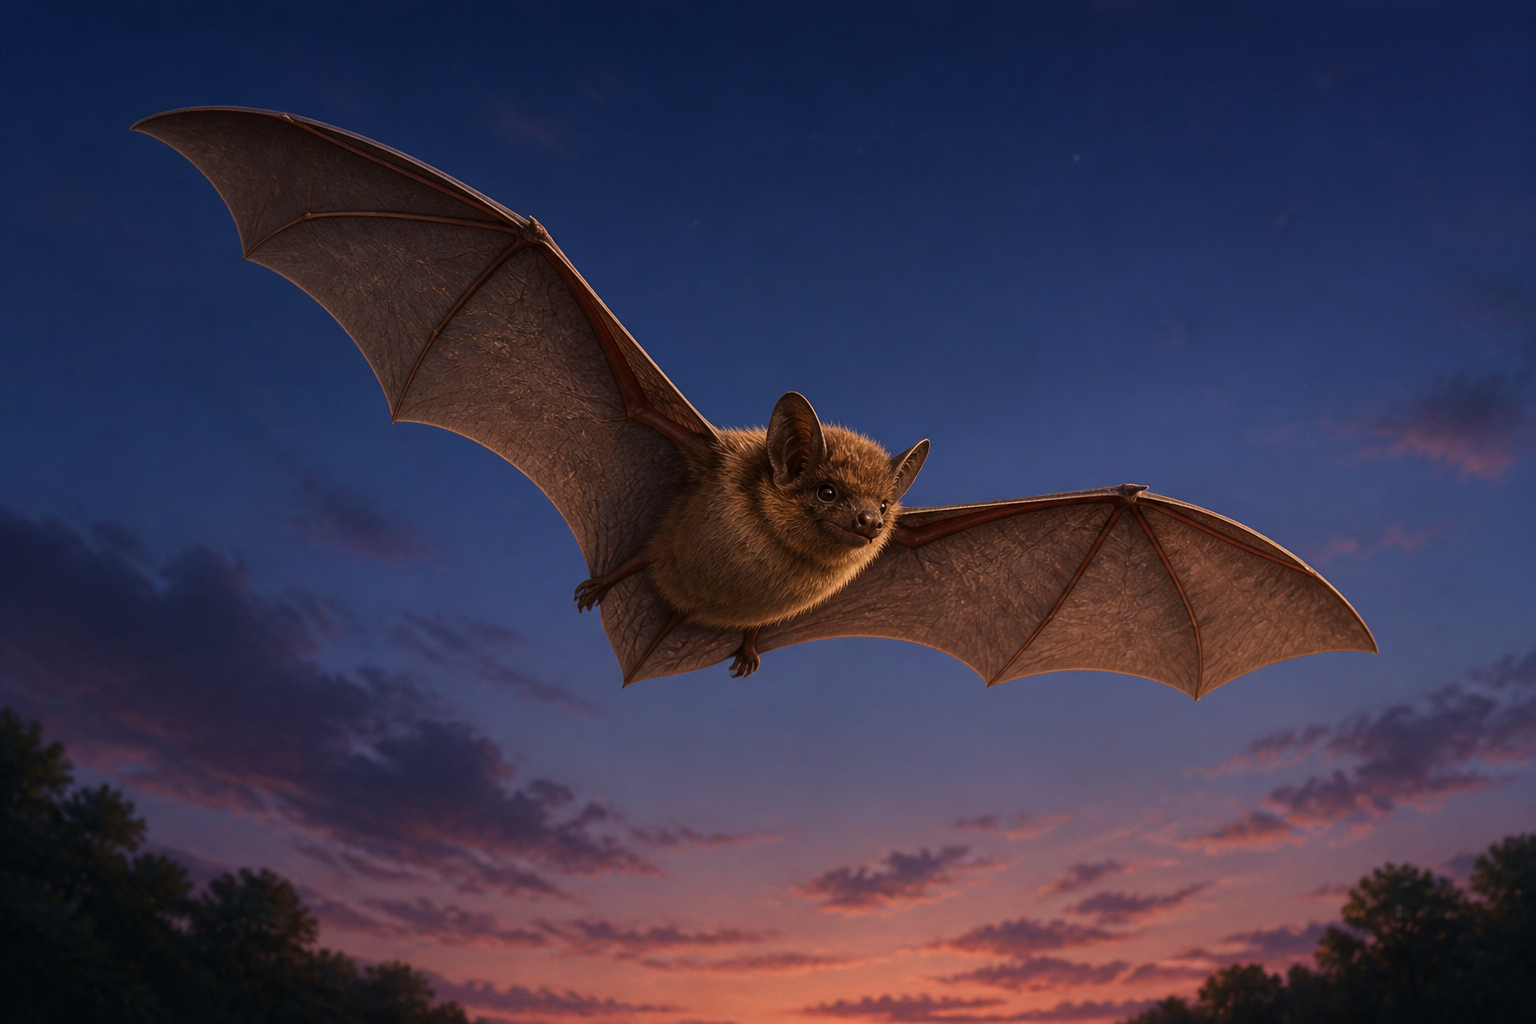
\includegraphics[width=0.6\linewidth]{images/book1/ai/g3-sort-bat.png}

{\small Elle vole comme un oiseau --- et porte des poils sur des
ailes nues~: la chauve-souris, l'épreuve classique du tri par
caractères plutôt que par impressions.}
\end{omfigure}

\begin{method}[Classer un animal inconnu]\label{met:g3:sorting-living-things:sort}
\begin{enumerate}
  \item Observe le corps~: \omterm{def:g1:the-five-senses:sense}{peau}, poils, \omterm{def:g1:animals-around-us:covering}{plumes} ou \omterm{def:g1:animals-around-us:covering}{écailles}~? combien
        de pattes~? des ailes~? un bec~?
  \item Renseigne-toi sur les petits si tu le peux~: du \omterm{def:g2:animals-grow-up:born}{lait}~? des
        \omterm{def:g2:animals-grow-up:born}{œufs}~? une étape de têtard~?
  \item Compare avec les groupes de
        \cref{prop:g3:sorting-living-things:groups} et place
        l'\omterm{def:g1:animals-around-us:animal}{animal} là où ses \emph{caractères} conviennent~;
  \item si une impression («~il vole~!~») contredit un caractère
        («~il a des poils~»), fie-toi au caractère.
\end{enumerate}
\end{method}

\section{On classe aussi les plantes}

\begin{proposition}[Classer les plantes]\label{prop:g3:sorting-living-things:plants}
Les \omterm{def:g1:plants-around-us:plant}{plantes} se trient par leurs caractères, tout comme les \omterm{def:g1:animals-around-us:animal}{animaux}.
Des \omterm{def:g3:sorting-living-things:criterion}{critères} utiles~: fait-elle des \emph{\omterm{def:g1:plants-around-us:parts}{fleurs}} et des \omterm{def:g2:from-seed-to-plant:seed}{graines} (la
pâquerette, le marronnier) ou jamais (la fougère, la mousse)~? Sa
\omterm{def:g1:plants-around-us:parts}{tige} est-elle tendre et verte, ou ligneuse comme le tronc d'un
\emph{arbre}~? Ses \omterm{def:g1:plants-around-us:parts}{feuilles} sont-elles larges, ou en aiguilles comme
celles du pin~?
\end{proposition}
\admitted

\begin{example}[Trois coins du parc]\label{ex:g3:sorting-living-things:park}
Dans un même parc~: le rosier --- des \omterm{def:g1:plants-around-us:parts}{fleurs}, des \omterm{def:g1:plants-around-us:parts}{tiges} ligneuses~;
la mousse du mur nord --- jamais de \omterm{def:g1:plants-around-us:parts}{fleurs}, pas de vraie \omterm{def:g1:plants-around-us:parts}{tige} du
tout~; le pin --- un arbre à aiguilles et à cônes. Trois \omterm{def:g1:plants-around-us:plant}{plantes},
trois réponses différentes aux mêmes \omterm{def:g3:sorting-living-things:criterion}{critères}.
\end{example}

\begin{remark}[Classer est le premier pas d'une science]\label{rem:g3:sorting-living-things:science}
Des groupes bien faits permettent de poser de meilleures questions~:
tout ce qui est vrai des \omterm{prop:g3:sorting-living-things:groups}{insectes} en général --- six pattes, un corps
en trois parties, souvent des ailes --- est d'un coup connu pour des
centaines de milliers d'espèces à la fois. Des chapitres plus tard
transformeront le tri en un arbre de parenté de tous les \omterm{def:g1:living-or-not:living}{êtres
vivants} --- pour l'instant, apprends à \omterm{def:g3:sorting-living-things:criterion}{trier} d'après ce que tu vois.
\end{remark}

\section{Exercices}

\begin{exercise}[$\star$]\label{exo:g3:sorting-living-things:1}
Qu'est-ce qu'un \omterm{def:g3:sorting-living-things:criterion}{critère}~? Donne un bon \omterm{def:g3:sorting-living-things:criterion}{critère} pour \omterm{def:g3:sorting-living-things:criterion}{trier} les
\omterm{def:g1:animals-around-us:animal}{animaux}, et un que les biologistes évitent.
\end{exercise}

\begin{exercise}[$\star$]\label{exo:g3:sorting-living-things:2}
Donne le caractère (ou les caractères) qui définit chaque groupe~:
\omterm{prop:g3:sorting-living-things:groups}{insectes}, \omterm{prop:g3:sorting-living-things:groups}{poissons}, \omterm{prop:g3:sorting-living-things:groups}{oiseaux}, \omterm{prop:g3:sorting-living-things:groups}{mammifères}.
\end{exercise}

\begin{exercise}[$\star$]\label{exo:g3:sorting-living-things:3}
Place chaque \omterm{def:g1:animals-around-us:animal}{animal} dans son groupe~: l'abeille, le poisson rouge,
l'autruche, la vache, la grenouille.
\end{exercise}

\begin{exercise}[$\star$]\label{exo:g3:sorting-living-things:4}
La chauve-souris vole. Pourquoi est-ce un mammifère et non un
oiseau~? Quels caractères décident~?
\end{exercise}

\begin{exercise}[$\star$]\label{exo:g3:sorting-living-things:5}
La baleine vit dans la mer. Pourquoi n'est-ce pas un poisson~? Quels
caractères décident~?
\end{exercise}

\begin{exercise}[$\star$]\label{exo:g3:sorting-living-things:6}
Une araignée a huit pattes. Peut-elle être un insecte~? Que répond
le \omterm{def:g3:sorting-living-things:criterion}{critère}~?
\end{exercise}

\begin{exercise}[$\star$]\label{exo:g3:sorting-living-things:7}
Trie ces \omterm{def:g1:plants-around-us:plant}{plantes} avec les \omterm{def:g3:sorting-living-things:criterion}{critères} de
\cref{prop:g3:sorting-living-things:plants}~: la pâquerette, la
mousse, le pin, le rosier.
\end{exercise}

\begin{exercise}[$\star$]\label{exo:g3:sorting-living-things:8}
À toi d'essayer~: trie les \omterm{def:g1:animals-around-us:animal}{animaux} de ta rue ou de ton jardin ---
tous ceux que tu repères en une promenade --- dans les groupes de ce
chapitre. Quel groupe l'emporte en nombre~?
\end{exercise}

\begin{exercise}[$\star\star$]\label{exo:g3:sorting-living-things:9}
Léa trie les \omterm{def:g1:animals-around-us:animal}{animaux} en «~\omterm{def:g1:animals-around-us:animal}{animaux} de compagnie~» et «~\omterm{def:g1:animals-around-us:animal}{animaux}
sauvages~». Son amie trie les mêmes \omterm{def:g1:animals-around-us:animal}{animaux} en «~\omterm{prop:g3:sorting-living-things:groups}{mammifères}~» et
«~\omterm{prop:g3:sorting-living-things:groups}{oiseaux}~». Quel tri est celui d'un biologiste, et pourquoi~?
Utilise \cref{rem:g3:sorting-living-things:why}.
\end{exercise}

\begin{exercise}[$\star\star$]\label{exo:g3:sorting-living-things:10}
Un manchot nage à merveille, ne vole pas, et il est couvert de ce
qui ressemble à des tuiles brillantes. Une naturaliste regarde de
plus près~: les «~tuiles~» sont des \omterm{def:g1:animals-around-us:covering}{plumes} serrées, et il y a un
bec. Applique
\cref{met:g3:sorting-living-things:sort} au manchot, étape par
étape.
\end{exercise}
